\documentclass{beamer}
%\usepackage{beamerthemeshadow}
\usepackage{graphicx}
\usepackage{amssymb}
\usepackage{amsmath}
\usepackage{eucal}
\usepackage{upgreek}




% special 
\usepackage{ifthen}
\usepackage{ifpdf}
\usepackage{float}
\usepackage{color}

% fonts
\usepackage{latexsym}
\usepackage{amsmath} 
\usepackage{amssymb} 
\usepackage{bm}
\usepackage{wasysym}


\ifpdf
\usepackage{graphicx}
\usepackage{epstopdf}
\else
\usepackage{graphicx}
\usepackage{epsfig}
\fi


%\usepackage[colorlinks,linkcolor=blue,bookmarks=true]{hyperref}

\renewcommand\mathfamilydefault{\rmdefault}

\graphicspath{{MSc_figures/},{../}, {PTA_figures/}}

%\usetheme{Madrid}
\usetheme{Boadilla}
\setbeamertemplate{navigation symbols}{}%remove navigation symbols

%%%%%%%%%%%%   dcohen cmds:

%%%%%%%%%%%%%%%%%%%%%%%%%%%%%%%%%%%%%%%%%%%%%%%%%%%%%%%%%%%%%%%%

% NEW 
\newcommand{\abs}[1]{\left|#1\right|}
\newcommand{\Prob}{\mbox{Prob}\,}
\newcommand{\erf}{\mbox{erf}\,}
\newcommand{\barline}[1]{#1}

% math symbols I
\newcommand{\sinc}{\mbox{sinc}}
\newcommand{\const}{\mbox{const}}
\newcommand{\trc}{\mbox{trace}}
\newcommand{\intt}{\int\!\!\!\!\int }
\newcommand{\ointt}{\int\!\!\!\!\int\!\!\!\!\!\circ\ }
\newcommand{\ar}{\mathsf r}
\newcommand{\im}{\mbox{Im}}
\newcommand{\re}{\mbox{Re}}

% math symbols II
\newcommand{\eexp}{\mbox{e}^}
\newcommand{\bra}{\left\langle}
\newcommand{\ket}{\right\rangle}

% Mass symbol
\newcommand{\mass}{\mathsf{m}} 
\newcommand{\Mass}{\mathsf{M}} 

% more math commands
\newcommand{\tbox}[1]{\mbox{\tiny #1}}
\newcommand{\bmsf}[1]{\bm{\mathsf{#1}}} 
%\newcommand{\amatrix}[1]{\matrix{#1}} 
\newcommand{\amatrix}[1]{\begin{matrix} #1 \end{matrix}} 
\newcommand{\pd}[2]{\frac{\partial #1}{\partial #2}}

% equations
\newcommand{\mylabel}[1]{\label{#1}} 
%\newcommand{\mylabel}[1]{\textcolor{blue}{[#1]}\label{#1}} 
\newcommand{\beq}{\begin{eqnarray}}
\newcommand{\eeq}{\end{eqnarray}} 
\newcommand{\be}[1]{\begin{eqnarray}\ifthenelse{#1=-1}{\nonumber}{\ifthenelse{#1=0}{}{\mylabel{e#1}}}}
\newcommand{\ee}{\end{eqnarray}} 

% arrangement
\newcommand{\drawline}{\begin{picture}(500,1)\line(1,0){500}\end{picture}}
\newcommand{\bitem}{$\bullet$ \ \ \ }
\newcommand{\Cn}[1]{\begin{center} #1 \end{center}}
\newcommand{\mpg}[2][1.0\hsize]{\begin{minipage}[b]{#1}{#2}\end{minipage}}
\newcommand{\mpgt}[2][1.0\hsize]{\begin{minipage}[t]{#1}{#2}\end{minipage}}
\newcommand{\putgraph}[2][width=0.30\hsize]{\includegraphics[#1]{#2}}

% more
%\newcommand{\Eq}[1]{Eq.\!\!~(\ref{#1})}
%\newcommand{\Fig}[1]{Fig.\!\!~\ref{#1}}  
\newcommand{\Eq}[1]{\textcolor{blue}{Eq.\!\!~(\ref{#1})}} 
\newcommand{\Fig}[1]{\textcolor{blue}{Fig.}\!\!~\ref{#1}} 
\newcommand{\hide}[1]{} %{\textcolor{red}{[hidden text]}} %{}
\newcommand{\rmrk}[1]{\textcolor{red}{#1}}


\begin{document}
\title[PhD Proposal]{Random matrix modelling of transport in sparse systems}  
\author{Yaron de Leeuw}
\institute{BGU}
\date{April 29, 2013} 

%%%%
\begin{frame}
 \titlepage
Advisor: Doron Cohen
\end{frame}

%%%%
%\begin{frame}
% \frametitle{Table of contents}
% \tableofcontents
%\end{frame}


%%%%%%
\begin{frame}
\frametitle{The model system}
\begin{columns}
    \begin{column}{0.6\textwidth}
    %
    Rate Equation:
    %
    \begin{align*}
      \frac{dp_n(t)}{dt} &= \sum_m w_{nm} p_m(t)\\
      w_{nm} \ \ &= \ \  w_0 \ \eexp{-\epsilon_{nm}} \ \eexp{-|x_n-x_m|/\xi}\\
      s &\equiv \frac{\xi}{r_0} \qquad \leftarrow \textrm{  Sparsity parameter}
    \end{align*}
    %
    %
    \begin{itemize}
    \item $\epsilon_{nm}>0$ is a random activation energy
    \item $x_n$ are the locations of sites in space
    \end{itemize}
    \end{column}
    \begin{column}{0.4\textwidth}
    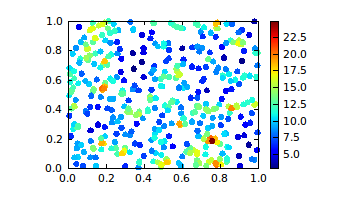
\includegraphics[width=1\hsize]{pts_points}
    \end{column}
\end{columns}

\[
\rho(r,\epsilon)drd\epsilon \ \ = \ \ \frac{\Omega_d \, r^{d-1}dr}{r_0^{d}} \ f(\epsilon)d\epsilon,     
\ \ \ \ \ \ \ \ \Omega_d=2,2\pi,4\pi
\]

The "degenerate" model -  $f(\epsilon) = \delta(\epsilon)$

The "Mott" hopping model - $f(\epsilon) = 1$
\end{frame}


%%%%%%%%%%%%%%%%%%%%%%%%%%%%%%%%%%%%%%%%%%%%%%%%%%%%%%%%%%%%%%%%%%%%%%%%
%%%%%%%%%%%%%%%%%%%%%%%%%%%%%%%%%%%%%%%%%%%%%%%%%%%%%%%%%%%%%%%%%%%%%%%%
\begin{frame}
    \frametitle{Diffusion coefficient}
    The long term dynamics are characterized by the spreading, the survival 
    probability and the spectral counting function. For diffusive systems:
    \vspace{16pt}

    \begin{align*}
        \text{long time spreading -} & &S(t) &= \left\langle r^2(t)\right\rangle \quad\sim\quad  (2d)Dt\ \\
        \text{long time survival -} & &\mathcal{P}(t) &\sim  \frac{1}{\left({D t}\right)^{d/2}}        \\
        \text{spectral density -} & &\mathcal{N}(\lambda)  &= \int^\lambda g(\lambda)d\lambda  \quad\sim\quad \left[\frac{\lambda}{D}\right]^{d/2} \\
    \end{align*}
    %
$D$ can be determined via  numerical solution of a circuit equation $GV=I$

or via the small $\lambda$ asymptote of $\mathcal{N}(\lambda)$.
    %
\end{frame}
%%%%%%%%%%%%%%%%%%%%%%%%%%%%%%%%%%%%%%%%%%%%%%%%%%%%%%%%%%%%%%%%%%%%%%%%
%%%%%%%%%%%%%%%%%%%%%%%%%%%%%%%%%%%%%%%%%%%%%%%%%%%%%%%%%%%%%%%%%%%%%%%%
\begin{frame}
\frametitle{Random site model, $1d$ vs $2d$}
\begin{columns}
\begin{column}{0.45\textwidth}
$d=1$, not sparse $s>1$:
\begin{align*}
D \ \ &=\ \  \frac{s -1 }{s} w_0, 
\end{align*}
$d=1$, sparse $s<1$  
%
\newline
\vspace{-15pt}
%\fcolorbox{red}{white}
{\begin{align*}S(t) \ \ \sim \ \ t^{2s/(1+s)}\end{align*}
}
\vspace{-20pt}
%
\begin{center}
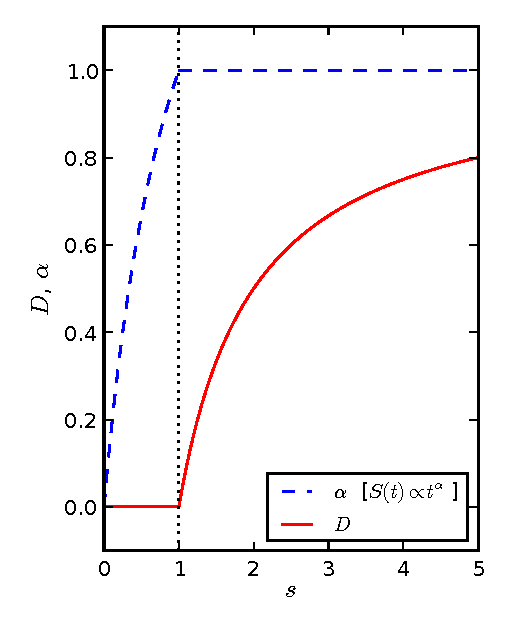
\includegraphics[width=0.6\hsize]{ptsD_1D_long}
\end{center}
\end{column}
\vrule{}
\begin{column}{0.55\textwidth}
$d=2$, always finite $D$.
\newline
%
\begin{align*}
D_{\textrm{ERH}} \ &= \ \textrm{EXP}_{d+2} \left( \frac{1}{s_{\textit{eff}}} \right)\eexp{-1/s_{\textit{eff}}} D_{\textrm{linear}}\\
s_{\textit{eff}} \ &= \ \left(\frac{d}{\Omega_d}n_c \right)^{-1/d} \frac{\xi}{r_0}
\end{align*}
\begin{center}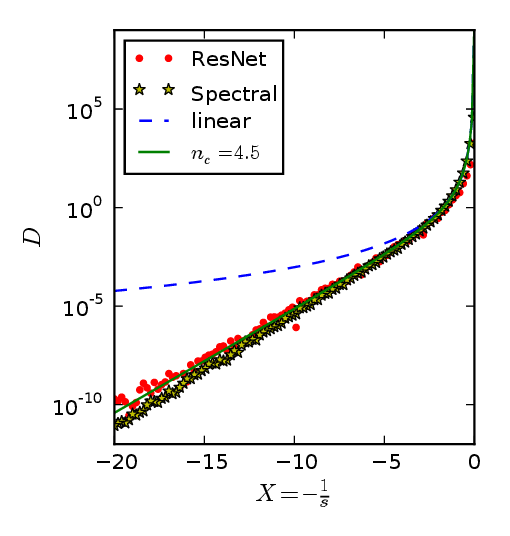
\includegraphics[width=0.6\hsize]{ptsD_2D_long}\end{center}
\end{column}
\end{columns}

\end{frame}
%%%%%%%%%%%%%%%%%%%%%%%%%%%%%%%%%%%%%%%%%%%%%%%%%%%%%%%%%%%%%%%%%%%%%%%%
%%%%%%%%%%%%%%%%%%%%%%%%%%%%%%%%%%%%%%%%%%%%%%%%%%%%%%%%%%%%%%%%%%%%%%%%
\begin{frame}
\frametitle{Spectral comparison $1d$ vs $2d$}

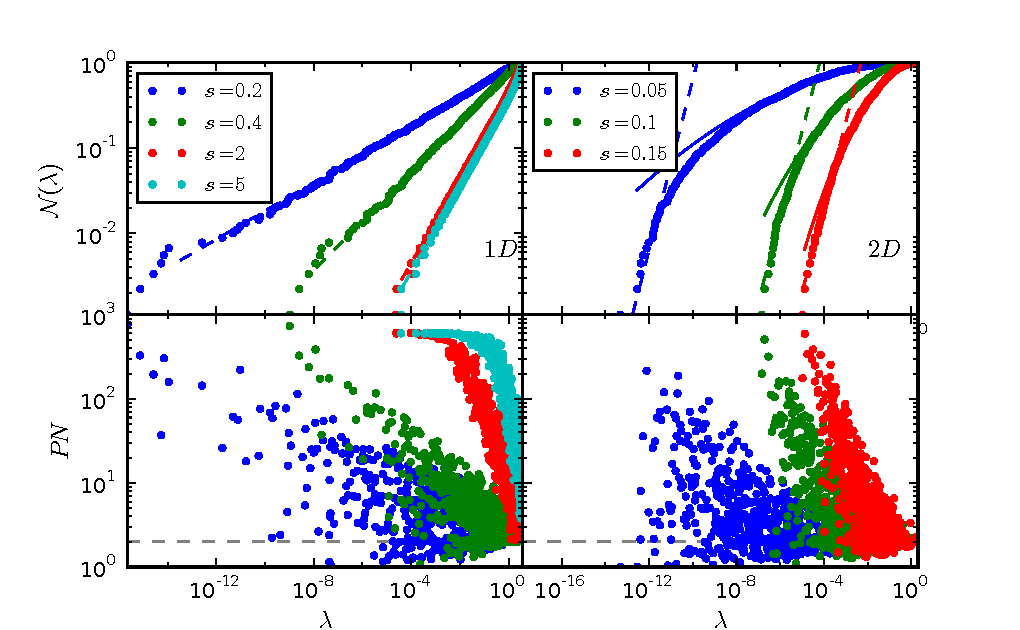
\includegraphics[width=0.90\hsize]{pts_Spectral_PN}

Solid lines - RG theory prediction [{\bf Amir, Oreg, Imry (2010)}].

Dashed lines  - Resistor network theory prediction [{\bf YdL, DC (2012)}].
\end{frame}
%%%%%%%%%%%%%%%%%%%%%%%%%%%%%%%%%%%%%%%%%%%%%%%%%%%%%%%%%%%%%%%%%%%%%%%%
%%%%%%%%%%%%%%%%%%%%%%%%%%%%%%%%%%%%%%%%%%%%%%%%%%%%%%%%%%%%%%%%%%%%%%%%
\begin{frame} \frametitle{Several views over localization in this model}
{ \fontfamily{lmr}\fontsize{8}{7.2}\selectfont
Localization in a disordered elastic medium near two dimensions\newline
Sajeev John, H. Sompolinsky, M.J. Stephen, Phys. Rev. B 27, 55925603 (1983)
\begin{itemize}
\item All states are localized
\item Localization length diverges for $\lambda \rightarrow 0$
\item Debye law holds (diffusion)
\end{itemize}
Localization, Anomalous Diffusion, and Slow Relaxations\newline
A. Amir, Y. Oreg, Y. Imry, Phys. Rev. Lett. 105, 070601 (2010)
\begin{itemize}
\item All states are localized
\item There is sub-diffusion rather than difussion
\end{itemize}
Diffusion in sparse networks: Linear to semilinear crossover \newline
Y. de Leeuw, D. Cohen, Phys. Rev. E 86, 051120 (2012)
\begin{itemize}
\item All states are localized
\item There is a percolation crossover at finite $\lambda$
\item Localization length diverges for $\lambda \rightarrow 0$
\item Debye law holds (diffusion)
\end{itemize}
Emergent percolation length and localization in random elastic networks \newline
A. Amir, J. J. Krich, V. Vitelli, Y. Oreg, Y. Imry, arXiv:1209.2169 (2012)
\begin{itemize}
\item There is an Anderson mobility edge at finite $\lambda$
\item The low lying states become de-localized
\item Debye law holds (diffusion)
\end{itemize}

}
\end{frame}
%%%%%%%%%%%%%%%%%%%%%%%%%%%%%%%%%%%%%%%%%%%%%%%%%%%%%%%%%%%%%%%%%%%%%%%%
%%%%%%%%%%%%%%%%%%%%%%%%%%%%%%%%%%%%%%%%%%%%%%%%%%%%%%%%%%%%%%%%%%%%%%%%
\begin{frame}\frametitle{Work plan}


\begin{itemize}
    \item Current goal:  find the relation between resistor network calculation and
    Fourier law, or between mesoscopic transport and heat transport.
    \begin{itemize}
        \item  Study and explain the band structure of banded-sparse models.
        \item  Calculate heat transport and resistor network transport 
               for these models, and look for similarities (e.g. VRH and percolation)
        \item  In the weak banded model, each energy $\lambda$ has
               more than one $k$: check the effects on scattering and 
               localization length calculations.
        \item  Check $N$ and $b$ scaling.
    \end{itemize}
    \item  Models with relaxation
    \item  Sinai spectrum in $1d$
    \item  Sinai diffusion in $2d$
    \item  Quantum spreading
    \item  Discrete particles (many-body physics)
\end{itemize}
\end{frame}
%%%%%%%%%%%%%%%%%%%%%%%%%%%%%%%%%%%%%%%%%%%%%%%%%%%%%%%%%%%%%%%%%%%%%%%%
%%%%%%%%%%%%%%%%%%%%%%%%%%%%%%%%%%%%%%%%%%%%%%%%%%%%%%%%%%%%%%%%%%%%%%%%
\begin{frame}\frametitle{Band structure for banded weak disorder}
We can analytically compute the spectrum for a banded matrix of ones (Bloch).

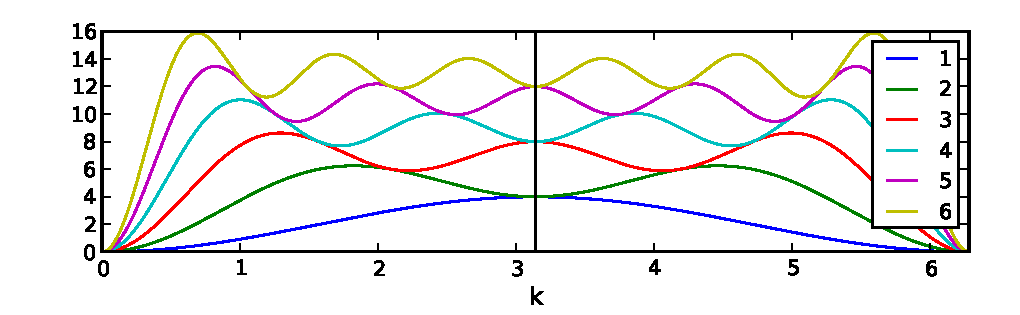
\includegraphics[width=0.9\textwidth]{pta_theor_banded_ev}\newline
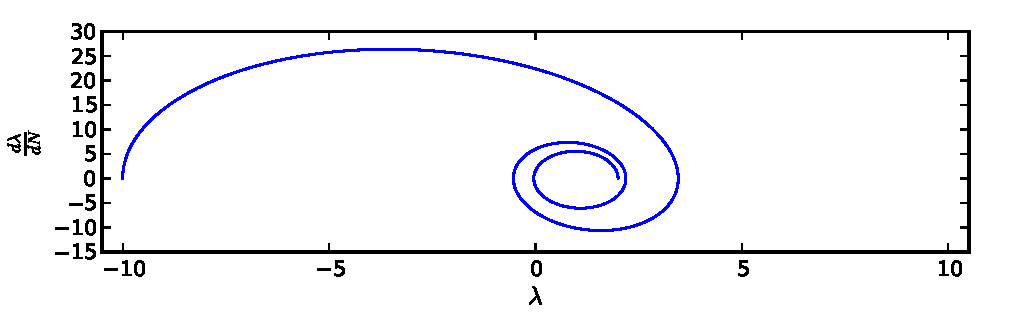
\includegraphics[width=0.9\textwidth]{pta_theor_banded_dos}

\end{frame}
%%%%%%%%%%%%%%%%%%%%%%%%%%%%%%%%%%%%%%%%%%%%%%%%%%%%%%%%%%%%%%%%%%%%%%%%
%%%%%%%%%%%%%%%%%%%%%%%%%%%%%%%%%%%%%%%%%%%%%%%%%%%%%%%%%%%%%%%%%%%%%%%%
\begin{frame}\frametitle{Band structure for banded weak disorder}

For weak disorder, $PN$ goes like $\textrm{DOS}^{-2}$ with the Bloch $\textrm{DOS}$

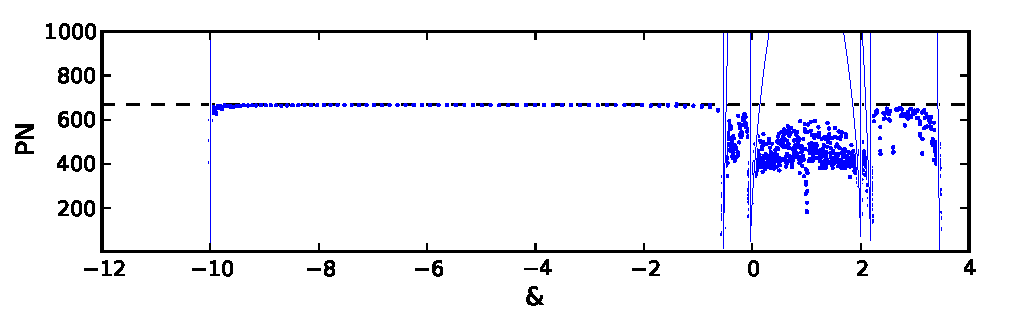
\includegraphics[width=0.9\textwidth]{pta_B_DD_low}

and $\mathcal{N}(\lambda)$ is very similar to the Bloch $\mathcal{N}(\lambda)$ (the dashed line)

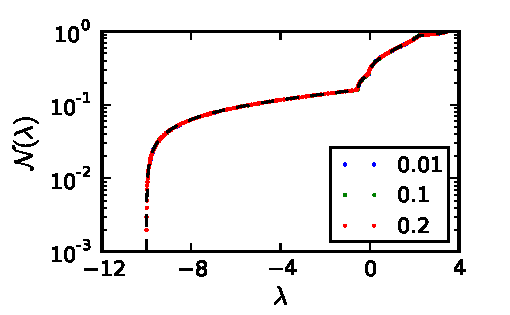
\includegraphics[width=0.45\textwidth]{pta_B_DD_low_ev}
\end{frame}
%%%%%%%%%%%%%%%%%%%%%%%%%%%%%%%%%%%%%%%%%%%%%%%%%%%%%%%%%%%%%%%%%%%%%%%%
%%%%%%%%%%%%%%%%%%%%%%%%%%%%%%%%%%%%%%%%%%%%%%%%%%%%%%%%%%%%%%%%%%%%%%%%
\begin{frame}\frametitle{$PN$ structure for random band}
\begin{center}
%\vspace{-20pt}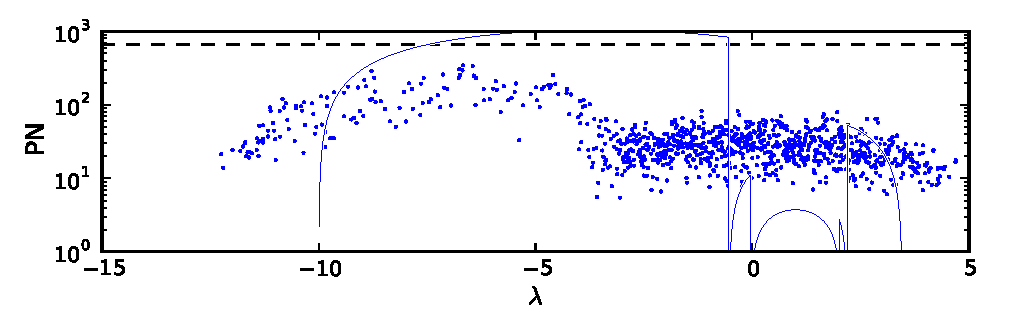
\includegraphics[width=0.60\textwidth]{pta_box2_positive}\newline
\vspace{-10pt}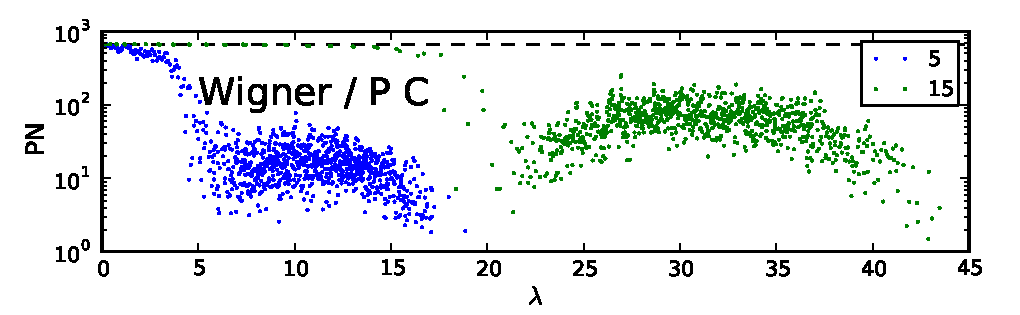
\includegraphics[width=0.60\textwidth]{pta_box2_pos_cons}\vspace{+5pt}\newline
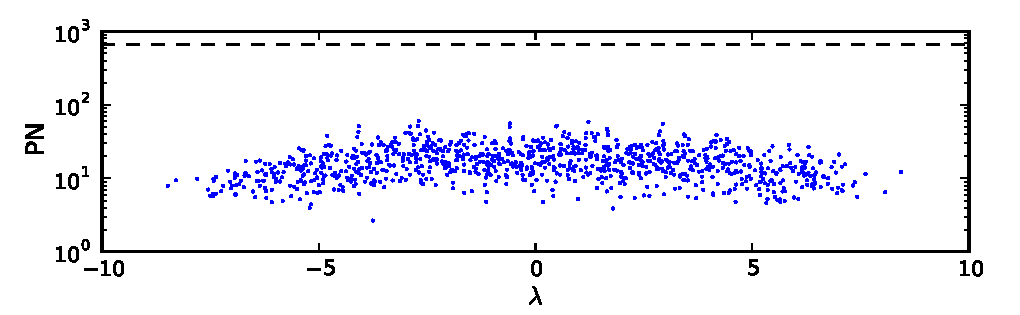
\includegraphics[width=0.60\textwidth]{pta_box2_symmetric}\newline
\vspace{-0pt}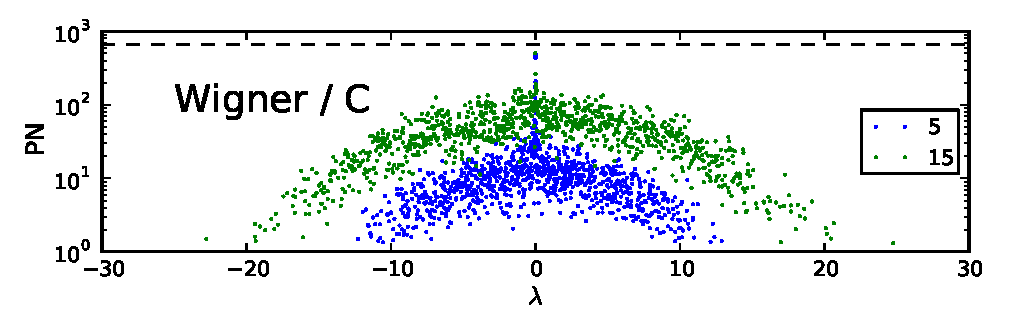
\includegraphics[width=0.60\textwidth]{pta_box2_sym_cons}\newline
\end{center}
\end{frame}
%%%%%%%%%%%%%%%%%%%%%%%%%%%%%%%%%%%%%%%%%%%%%%%%%%%%%%%%%%%%%%%%%%%%%%%%
%%%%%%%%%%%%%%%%%%%%%%%%%%%%%%%%%%%%%%%%%%%%%%%%%%%%%%%%%%%%%%%%%%%%%%%%
\begin{frame}\frametitle{$PN$ structure for banded - sparse model}
\begin{center}
%\vspace{-20pt}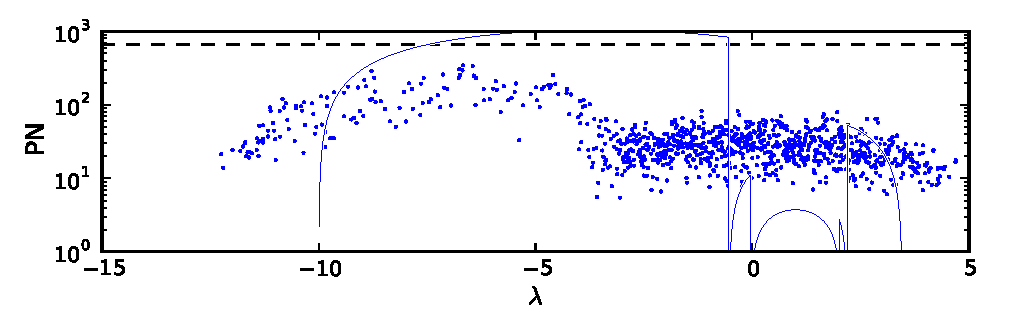
\includegraphics[width=0.60\textwidth]{pta_box2_positive}\newline
\vspace{-20pt}

\begin{align*}
w_{nm} =
\exp([-\eta, 0]) 
\end{align*}
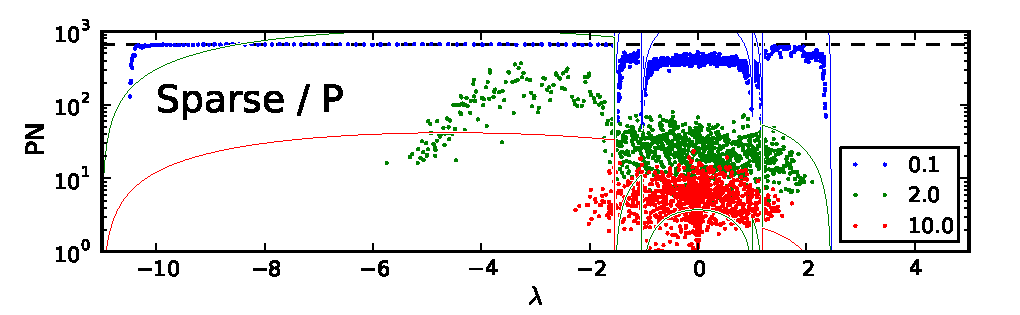
\includegraphics[width=0.60\textwidth]{pta_exp_regular}\newline
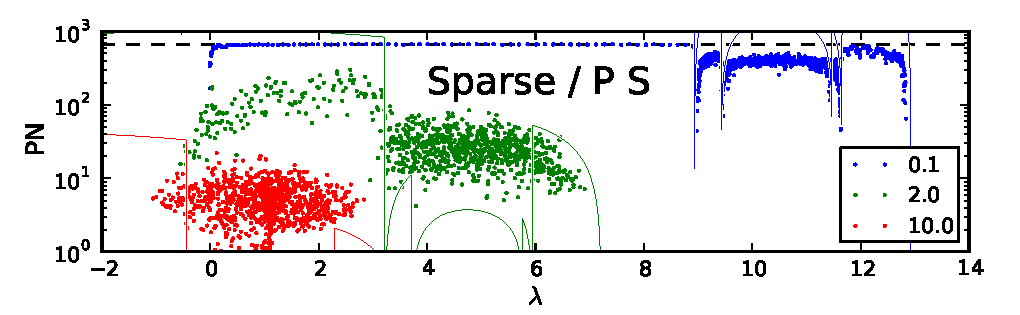
\includegraphics[width=0.60\textwidth]{pta_exp_shift}\newline
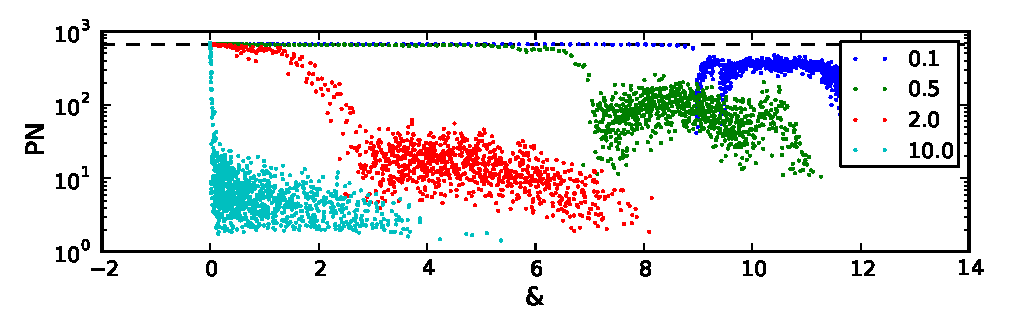
\includegraphics[width=0.60\textwidth]{pta_exp_cons}\newline
\end{center}
\end{frame}
\end{document}


